% Created 2017-03-28 Tue 11:02
\documentclass[t,10pt]{beamer}
\usepackage[utf8]{inputenc}
\usepackage[T1]{fontenc}
\usepackage{fixltx2e}
\usepackage{graphicx}
\usepackage{grffile}
\usepackage{longtable}
\usepackage{wrapfig}
\usepackage{rotating}
\usepackage[normalem]{ulem}
\usepackage{amsmath}
\usepackage{textcomp}
\usepackage{amssymb}
\usepackage{capt-of}
\usepackage{hyperref}
\usepackage{color}
\usepackage{listings}
\mode<beamer>{\usetheme{Madrid}}
\lstset{
language=sh,
otherkeywords={=, +, [, ], (, ), \{, \}, *, $},
emph={addgroup,adduser,alias,ant,apropos,apt-get,aptitude,aspell,awk,basename,bash,bc,bg,break,builtin,bzip2,cal,case,cat,cd,cfdisk,chgrp,chkconfig,chmod,chown,chroot,cksum,clear,cmp,comm,command,continue,cp,cron,crontab,csplit,cut,date,dc,dd,ddrescue,declare,df,diff,diff3,    dig,dir,dircolors,dirname,dirs,dmesg,du,echo,egrep,eject,enable,env,    ethtool,eval,exec,exit,expand,expect,export,expr,false,fdformat,    fdisk,fg,fgrep,file,find,fmt,fold,for,format,free,fsck,ftp,function,    fuser,gawk,getopts,    git,    grep,groups,gzip,    gunzip,    ,hash,head,help,history,hostname,    id,if,ifconfig,ifdown,ifup,import,install,    java, java6, java_cur    join,kill,killall,    let,ln,local,locate,logname,logout,look,lpc,lpr,lprint,lprintd,    lprintq,lprm,ls,lsof,make,man,mkdir,mkfifo,mkisofs,mknod,mmv,more,    mount,mtools,mtr,mv,    mysql,    netstat,nice,nl,nohup,notify-send,    noweb,noweave,    nslookup,op,    open,passwd,paste,pathchk,ping,pkill,popd,pr,printcap,printenv,    printf,ps,pushd,pwd,quota,quotacheck,quotactl,ram,rcp,read,    readarray,readonly,reboot,remsync,rename,renice,return,rev,rm,rmdir,    rsync,scp,screen,sdiff,sed,select,seq,set,sftp,shift,shopt,shutdown,    sleep,slocate,sort,source,split,ssh,strace,su,sudo,sum,    svn, svn2git,    symlink,sync,    tail,tar,tee,test,time,times,top,touch,tr,traceroute,trap,true,    tsort,tty,type,ulimit,umask,umount,unalias,uname,unexpand,uniq,    units,    unrar,    unset,unshar,until,useradd,usermod,users,uudecode,uuencode,    vdir,vi,vmstat,watch,wc,Wget,whereis,which,while,who,whoami,write,    zcat},
breaklines=true,
keywordstyle=\color{blue},
stringstyle=\color{red},
emphstyle=\color{black}\bfseries,
commentstyle=\color{gray}\slshape
}
\hypersetup{colorlinks=true, linkcolor=blue}
\AtBeginSection[]{\begin{frame}<beamer>\frametitle{Topic}\tableofcontents[currentsection]\end{frame}}
\lstset{basicstyle=\tiny\ttfamily}
\usetheme{Madrid}
\author{Stephen A. Sefick}
\date{2017-03-28}
\title{Getting Genomics Done with R}
\titlegraphic{\vspace{0.75in}
\includegraphics[width=0.5\textwidth,height=.1\textheight]{figures/comb_2.png}}
\hypersetup{
 pdfauthor={Stephen A. Sefick},
 pdftitle={Getting Genomics Done with R},
 pdfkeywords={},
 pdfsubject={},
 pdfcreator={Emacs 24.5.1 (Org mode 8.3.6)}, 
 pdflang={English}}
\begin{document}

\maketitle
\begin{frame}{Outline}
\tableofcontents
\end{frame}



\section{Introduction}
\label{sec:orgheadline4}
\begin{frame}[label={sec:orgheadline1}]{Motivation}
\begin{enumerate}[<+->]
\item How to arrive at analysis ready variants?
\item GATK HaplotypeCaller is "permissive"
\begin{itemize}
\item False Positives
\end{itemize}
\item How to separate True/False Positives
\begin{itemize}
\item classification/machine learning
\item \alert{filtering}
\item both
\end{itemize}
\item What software to use?
\begin{itemize}
\item \href{https://cran.r-project.org/}{R}
\item \href{https://bioconductor.org/}{Bioconductor Project}
\end{itemize}
\end{enumerate}
\end{frame}

\begin{frame}[label={sec:orgheadline2}]{Bioconductor}
\begin{enumerate}[<+->]
\item CRAN
\item Bioconductor- additional software repository
\item "Open Source Software For Bioinformatics"
\begin{itemize}
\item DNA micro-array
\item sequence
\item SNP
\item etc.
\end{itemize}
\item started 2001
\item 1294 user contributed packages
\end{enumerate}
\end{frame}

\begin{frame}[label={sec:orgheadline3}]{Bioconductor Packages}
\begin{enumerate}[<+->]
\item Installation similar to CRAN packages (\alert{automatic dependency resolution})
\begin{itemize}
\item Install/update Bioconductor
\begin{itemize}
\item source("\url{https://bioconductor.org/biocLite.R}")
\item biocLite()
\end{itemize}
\item Install packages
\begin{itemize}
\item biocLite("VariantAnnotation")
\end{itemize}
\end{itemize}
\item Documentation familiar and excellent
\item In addition, most packages have vignettes
\begin{itemize}
\item Vignettes are short "how-tos"
\end{itemize}
\item Most object oriented providing consistent "feel" for bioconductor packages
\begin{itemize}
\item CRAN mix of no OO, S3, S4, and newer R6
\item Flexibility is R's strength and weakness
\end{itemize}
\item \url{https://bioconductor.org/}
\end{enumerate}
\end{frame}


\section{VCF Annotations}
\label{sec:orgheadline17}
\begin{frame}[label={sec:orgheadline5}]{GATK Haplotype Caller Annotations}
\begin{enumerate}[<+->]
\item HaplotypeCaller includes/calculates annotations
\begin{itemize}
\item VCFs have a number of annotations
\begin{itemize}
\item e.g., genotype quality, depth, etc.
\end{itemize}
\end{itemize}
\item Annotations change
\begin{itemize}
\item e.g., HaplotypeCaller's gVCFs with Reference Genotype Quality
\item \href{https://software.broadinstitute.org/gatk/documentation/tooldocs/current/org_broadinstitute_gatk_tools_walkers_annotator_VariantAnnotator}{Custom annotations}
\end{itemize}
\item How do we use annotations?
\begin{itemize}
\item understanding the data
\item filtering
\item classification/machine learning
\end{itemize}
\item Non-model systems analysis ready variants
\begin{itemize}
\item hard-filtered call set
\item Bootstrapped Variant Quality Score Re-calibration (VQSR) call set using HF as training/truth data
\end{itemize}
\item Today concentrate on hard-filtering SNPs
\end{enumerate}
\end{frame}

\begin{frame}[label={sec:orgheadline6}]{Hard-filtering}
\begin{enumerate}[<+->]
\item Context specific
\begin{itemize}
\item SNPs
\item INDELs
\end{itemize}
\item GATK hard-filtering recommendations
\item These are \alert{recommendations}, developed with \alert{human} data, and might/likely will need to be modified based on the data
\end{enumerate}
\only<5>{
\begin{center}
\begin{tabular}{lrll}
\hline
\alert{Variant} & \# & \alert{Annotation} & \alert{Remove If}\\
\hline
\alert{Both} & 1 & DP & min=empirical; max=5 or 6 sigma\\
 & 2 & GQ (or RGQ) & empirical\\
\hline
\alert{SNP} & 3 & QD & < 2.0\\
 & 4 & MQ & < 40\\
 & 5 & FS & > 60\\
 & 6 & SOR & > 3.0\\
 & 7 & MQRankSum & < -12.5\\
 & 8 & ReadPosRankSum & < -8.0\\
\hline
\end{tabular}
\end{center}
}
\end{frame}

\begin{frame}[label={sec:orgheadline7}]{1 Depth (DP) - Depth of coverage}
\begin{enumerate}[<+->]
\item Min - no empirical guidance- look at plots
\item Max - 5 or 6x the standard deviation
\item How many reads cover a position
\begin{itemize}
\item GATK Caveat- slightly different from \alert{raw} depth of coverage
\item QC of the caller will remove reads (MAQ)
\end{itemize}
\end{enumerate}
\end{frame}

\begin{frame}[label={sec:orgheadline8}]{1 Depth (DP) - Depth of coverage}
\vspace{-15.5pt}
\begin{columns}
\begin{column}{0.5\columnwidth}
\begin{block}{Mitochondria}
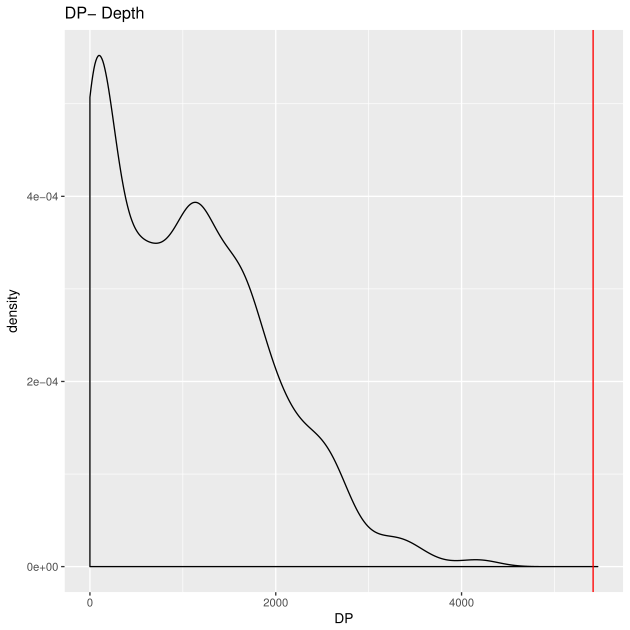
\includegraphics[width=6cm,height=6cm]{figures/chrM/document-page7.png}
\end{block}
\end{column}
\begin{column}{0.5\columnwidth}
\begin{block}{Chr1-20 and X}
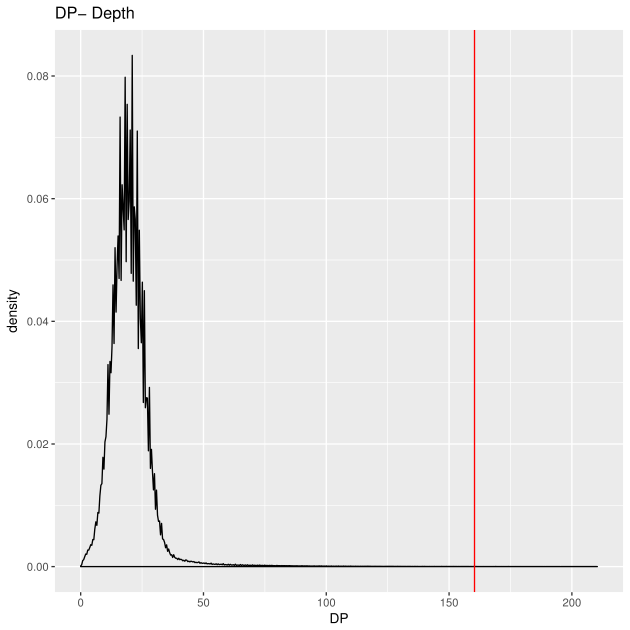
\includegraphics[width=6cm,height=6cm]{figures/NO_chrM/document-page7.png}
\end{block}
\end{column}
\end{columns}
\end{frame}


\begin{frame}[label={sec:orgheadline9}]{2 Genotype quality (GQ); Reference GQ (RGQ)}
\begin{enumerate}
\item Phred scaled probability of incorrect genotype
\begin{itemize}
\item 20 - 0.01; 30 - 0.001; 40 - 0.0001
\end{itemize}
\end{enumerate}
\vspace{-15.5pt}
\begin{columns}
\begin{column}{0.5\columnwidth}
\begin{block}{Mitochondria}
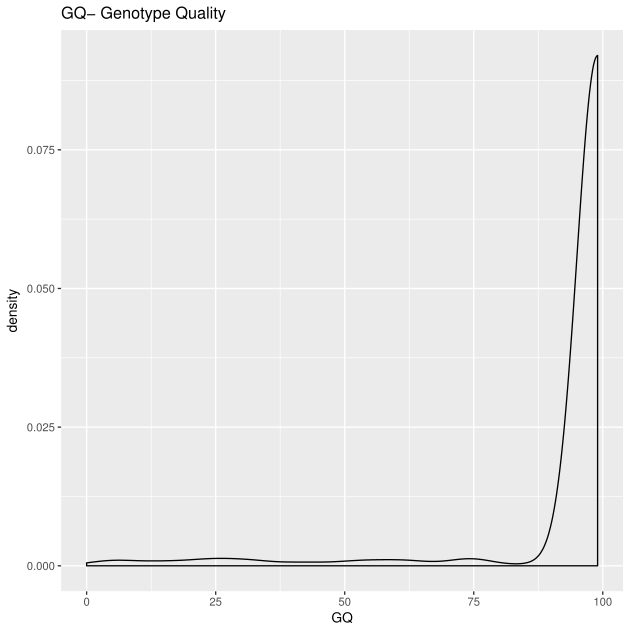
\includegraphics[width=6cm,height=6cm]{figures/chrM/document-page6.png}
\end{block}
\end{column}
\begin{column}{0.5\columnwidth}
\begin{block}{Chr1-20 and X}
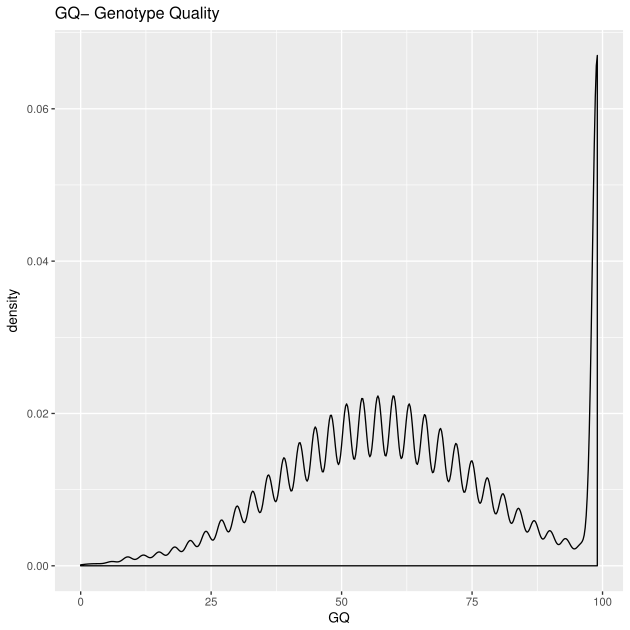
\includegraphics[width=6cm,height=6cm]{figures/NO_chrM/document-page6.png}
\end{block}
\end{column}
\end{columns}
\end{frame}



\begin{frame}[label={sec:orgheadline10}]{3 Variant quality/allele depth (QD)}
\begin{enumerate}
\item Variant Quality (QUAL) is the phred scaled probability that the variant is wrong.
\item allele depth is actual depth of each observed allele (How many actual reads; in contrast to \alert{DP}).
\end{enumerate}
\only<1>{
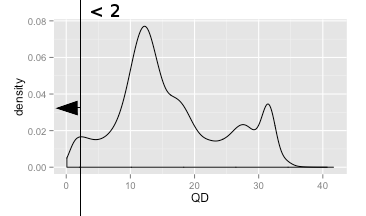
\includegraphics[width=.9\linewidth]{figures/Annotations_VQSR_GATK/ann_graphs/QD_ann.png} 
}\only<2>{
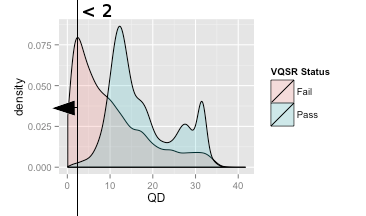
\includegraphics[width=.9\linewidth]{figures/Annotations_VQSR_GATK/ann_graphs/QD_VQSR_ann.png}   
}
\end{frame}

\begin{frame}[label={sec:orgheadline11}]{4 Root mean square mapping quality (MQ)}
\begin{enumerate}
\item phred scaled probability that the mapping position is wrong
\end{enumerate}
\only<1>{
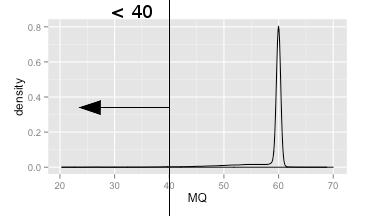
\includegraphics[width=.9\linewidth]{figures/Annotations_VQSR_GATK/ann_graphs/MQ_ann.png}   
}\only<2>{
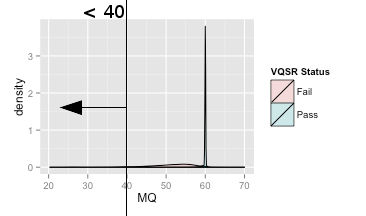
\includegraphics[width=.9\linewidth]{figures/Annotations_VQSR_GATK/ann_graphs/MQ_VQSR_ann.png}   
}
\end{frame}

\begin{frame}[label={sec:orgheadline12}]{5 Fisher strand bias (FS)}
\begin{enumerate}
\item phred scaled probability ALT on forward or reverse strand more or less than REF
\end{enumerate}
\only<1>{
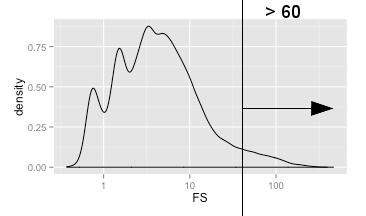
\includegraphics[width=.9\linewidth]{figures/Annotations_VQSR_GATK/ann_graphs/FS_ann.png}
}\only<2>{
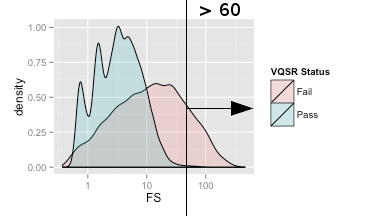
\includegraphics[width=.9\linewidth]{figures/Annotations_VQSR_GATK/ann_graphs/FS_VQSR_ann.png}
}
\end{frame}

\begin{frame}[label={sec:orgheadline13}]{6 Strand odds ratio (SOR)}
\begin{enumerate}
\item similar to FS, but updated for high coverage (NGS)   
\begin{itemize}
\item Ratio of reads that cover both alleles
\end{itemize}
\end{enumerate}
\only<1>{
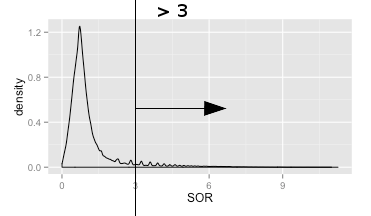
\includegraphics[width=.9\linewidth]{figures/Annotations_VQSR_GATK/ann_graphs/SOR_ann.png}
}\only<2>{
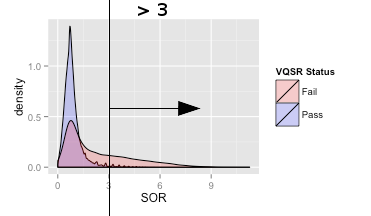
\includegraphics[width=.9\linewidth]{figures/Annotations_VQSR_GATK/ann_graphs/SOR_VQSR_ann.png}
}
\end{frame}

\begin{frame}[label={sec:orgheadline14}]{7 MQ rank sum test (MQRankSum)}
\begin{enumerate}
\item test compares MAQ ALT to REF
\begin{itemize}
\item (-) Alt lower MAQ
\item (+) Ref lower MAQ
\end{itemize}
\end{enumerate}
\only<1>{
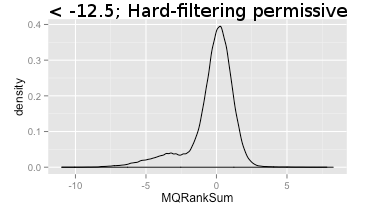
\includegraphics[width=.9\linewidth]{figures/Annotations_VQSR_GATK/ann_graphs/MQRankSum_ann.png}
}\only<2>{
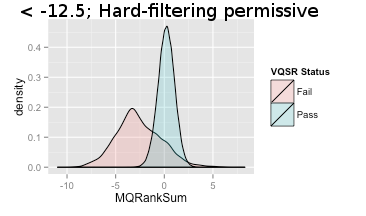
\includegraphics[width=.9\linewidth]{figures/Annotations_VQSR_GATK/ann_graphs/MQRankSum_VQSR_ann.png}
}
\end{frame}

\begin{frame}[label={sec:orgheadline15}]{8 Read position rank sum test (ReadPosRankSum)}
\begin{enumerate}
\item test for positional effects 
\begin{itemize}
\item (-) Alt close to end of read
\item (+) Ref close to end of read
\end{itemize}
\end{enumerate}
\only<1>{
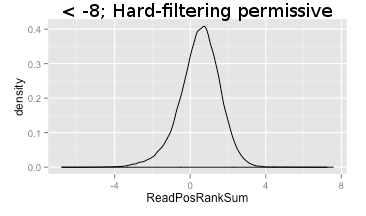
\includegraphics[width=.9\linewidth]{figures/Annotations_VQSR_GATK/ann_graphs/ReadPosRankSum_ann.png}
}\only<2>{
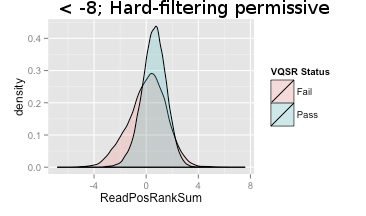
\includegraphics[width=.9\linewidth]{figures/Annotations_VQSR_GATK/ann_graphs/ReadPosRankSum_VQSR_ann.png}
}
\end{frame}

\begin{frame}[label={sec:orgheadline16}]{Hard-filtering Summary (SNPs and INDELS)}
\begin{center}
\begin{tabular}{lll}
\hline
\alert{Variant} & \alert{Annotation} & \alert{Remove If}\\
\hline
\alert{Both} & DP & min=empirical; max=5 or 6 sigma\\
 & GQ (or RGQ) & empirical\\
\hline
\alert{SNP} & QD & < 2.0\\
 & MQ & < 40\\
 & FS & > 60\\
 & SOR & > 3.0\\
 & MQRankSum & < -12.5\\
 & ReadPosRankSum & < -8.0\\
\hline
\alert{INDELs} & QD & < 2.0\\
 & ReadPosRankSum & < -20.0\\
 & InbreedingCoeff (> 10 samples) & < -8.0\\
 & FS & < 200.0\\
 & SOR & > 10.0\\
\hline
\end{tabular}
\end{center}
\end{frame}


\section{Using R/Bioconductor to filter vcf}
\label{sec:orgheadline19}
\begin{frame}[label={sec:orgheadline18}]{Variant Annotation}
\begin{enumerate}[<+->]
\item Could write a script in favorite language. 
\begin{itemize}
\item Know exactly what you did (+)
\item Time spent engineering software (-)
\end{itemize}
\item Hard Work already done
\begin{itemize}
\item Bioconductor
\item \href{https://bioconductor.org/packages/release/bioc/html/VariantAnnotation.html}{VariantAnnotation} 
\begin{itemize}
\item general parsing and filtering
\end{itemize}
\end{itemize}
\item Consistent interface
\begin{itemize}
\item Learn 1 piece of software and reuse
\end{itemize}
\item Custom filters
\begin{itemize}
\item flexible annotations (e.g., RGQ)
\item New annotations just "\alert{show up}"
\end{itemize}
\end{enumerate}
\end{frame}
\section{Exercise (HW 7)}
\label{sec:orgheadline21}
\begin{frame}[fragile,label={sec:orgheadline20}]{Extract, Filter, and Plot}
 \begin{enumerate}
\item Exercise folder on asc
\begin{itemize}
\item Scripts: 1\_initial\_annotation\_plot.sh; 2\_filter\_and\_plot.sh
\item Data: D\_PseudoFS14\_16
\item \href{https://github.com/ssefick/UsefulBioinformaticScripts}{UsefulBioinformaticScripts}
\end{itemize}
\item Edit "Variables" in 1\_initial\_annotation\_plot.sh
\lstset{language=sh,label= ,caption= ,captionpos=b,numbers=none}
\begin{lstlisting}
script_dir=${HOME}/Exercise/UsefulBioinformaticScripts           
data_dir=${HOME}/Exercise/D_PseudoFS14_16
out_dir=${HOME}/Exercise
\end{lstlisting}

\item save script and run
\item Inspect graphs and decide upon filtering thresholds
\item add variable definitions in \alert{2} to 2\_filter\_and\_plot.sh
\item Edit
\lstset{language=sh,label= ,caption= ,captionpos=b,numbers=none}
\begin{lstlisting}
#################################################################################  
##Filtering Parameters                                                             
##this is                                                                          
${script_dir}/filter_SNPs_GATK_hard_filter.CHUNKS.R -I ${out_dir}/${vcf1}.gz -T    
${out_dir}/${vcf1}.gz.tbi -O ${out_dir}/${vcf1}.filtered.vcf -C 10000 --QD=2       
--FS=60 --SOR=3 --MQRankSum=-8 --min_Depth=4 --max_Depth=32 --Genotype_Quality=20  

${script_dir}/filter_SNPs_GATK_hard_filter.CHUNKS.R -I ${out_dir}/${vcf2}.gz -T    
${out_dir}/${vcf2}.gz.tbi -O ${out_dir}/${vcf2}.filtered.vcf -C 10000 --QD=2       
--FS=60 --SOR=3 --MQRankSum=-8 --min_Depth=4 --max_Depth=32 --Genotype_Quality=20
\end{lstlisting}
\item save script and run
\item inspect graphs and write up.
\end{enumerate}
\end{frame}
\end{document}
